\documentclass[10pt]{article}
\usepackage{amscd,amsfonts,amssymb,amstext,latexsym} 
\usepackage{amsmath,mathbbol,mathrsfs,stmaryrd, mathtools} 
%\usepackage{mathbbol,mathrsfs,stmaryrd}
\usepackage {algorithm2e} 
\usepackage{theoremref}
\usepackage{dashrule}
\usepackage{booktabs}
\usepackage{float}
\usepackage[T1]{fontenc}
\usepackage[english]{babel} 
\usepackage {enumerate}
\usepackage{url}
%\usepackage {algpseudocode}  
\usepackage{graphics} 
\usepackage{tikz}
% \usepackage[square]{natbib}
\usepackage[]{geometry}
\usetikzlibrary{automata,calc}
%\usepackage{tgtermes} 
\usepackage{listings}
\usepackage{mathptmx}
\usepackage{fancyhdr}
\usepackage{verbatim}
\usepackage{enumitem}
\usepackage{booktabs}
\usepackage[flushleft]{threeparttable}
\usepackage{listings}
\usepackage{verbatim}
\usepackage{fancyhdr}
\usepackage{multirow,multicol}
\usepackage[colorlinks=true,linkcolor=blue,citecolor=black,urlcolor=black]{hyperref}
\usepackage{tabto}
\usepackage{xcolor}
\makeatletter
\newcommand*{\centerfloat}{%
  \parindent \z@
  \leftskip \z@ \@plus 1fil \@minus \textwidth
  \rightskip\leftskip
  \parfillskip \z@skip}
\makeatother
\definecolor{commentgreen}{RGB}{2,112,10}

%\graphicspath{{../../pics/}}
\fancypagestyle{plain}{
\fancyhf{}
\rhead{School of Computer Science and Applied Mathematics\\ 
%\noindent\rule{15.4cm}{0.4pt}\\
\footnotesize{\textsc{University of the Witwatersrand, Johannesburg}}}
\lhead{
\includegraphics[scale=0.08]{./witslogo_h.png}}
\fancyfoot[C]{\thepage}
\renewcommand{\headrulewidth}{0.4pt}
}

\textwidth=16.8cm 
\textheight=21.0cm 
\evensidemargin 0pt 
\oddsidemargin 0pt 
\leftmargin 0pt 
\rightmargin 0pt 
\setlength{\topmargin}{-20pt} 
\setlength{\footskip}{30pt}
\setlength{\parindent}{0pt}
\setlength{\parskip}{1em}
\linespread{1} 
% 
\makeatletter
\newcommand{\rmnum}[1]{\romannumeral #1}
\newcommand{\Rmnum}[1]{\expandafter\@slowromancap\romannumeral #1@}
\makeatother
\pagenumbering{arabic}
\usepackage{etoolbox}
\makeatletter

\pretocmd{\NAT@citex}{%
  \let\NAT@hyper@\NAT@hyper@citex
  \def\NAT@postnote{#2}%
  \setcounter{NAT@total@cites}{0}%
  \setcounter{NAT@count@cites}{0}%
  \forcsvlist{\stepcounter{NAT@total@cites}\@gobble}{#3}}{}{}
\newcounter{NAT@total@cites}
\newcounter{NAT@count@cites}
\def\NAT@postnote{}

% include postnote and \citet closing bracket in hyperlink
\def\NAT@hyper@citex#1{%
  \stepcounter{NAT@count@cites}%
  \hyper@natlinkstart{\@citeb\@extra@b@citeb}#1%
  \ifnumequal{\value{NAT@count@cites}}{\value{NAT@total@cites}}
    {\ifNAT@swa\else\if*\NAT@postnote*\else%
     \NAT@cmt\NAT@postnote\global\def\NAT@postnote{}\fi\fi}{}%
  \ifNAT@swa\else\if\relax\NAT@date\relax
  \else\NAT@@close\global\let\NAT@nm\@empty\fi\fi% avoid compact citations
  \hyper@natlinkend}
\renewcommand\hyper@natlinkbreak[2]{#1}

% avoid extraneous postnotes, closing brackets
\patchcmd{\NAT@citex}
  {\ifNAT@swa\else\if*#2*\else\NAT@cmt#2\fi
   \if\relax\NAT@date\relax\else\NAT@@close\fi\fi}{}{}{}
\patchcmd{\NAT@citex}
  {\if\relax\NAT@date\relax\NAT@def@citea\else\NAT@def@citea@close\fi}
  {\if\relax\NAT@date\relax\NAT@def@citea\else\NAT@def@citea@space\fi}{}{}

\makeatother
\usepackage{moreverb} 
\usepackage{natbib}
\bibliographystyle{named-wits}
\begin{document}

\title{AI RBC REPORT \\ 
}
\author{Sayfullah Jumoorty (2430888) \\ \\ Muhammed Muaaz Dawood (2425639) \\ \\ Mujammil Mohsin Gulam Sakhidas (2436109)}
% \date{Put your submission date here}
\maketitle 
\pagestyle{fancy}
\fancyhf{}
\fancyhead[R]{\thepage}
\fancyhead[L]{COMS4057A}
\pagenumbering{arabic} 

\begin{figure}[H]
\centering

\includegraphics[width=0.5\textwidth]{logo-round.png}
\label{fig:LOGO}
\end{figure}

\newpage

\tableofcontents

\newpage

\section{Introduction}

This report outlines the development and performance evaluation of an agent tailored for Reconnaissance Blind Chess (RBC). In this strategic pursuit, the agent's construction demanded smart planning. Through a systematic approach, this document elucidates the agent's design methodologies, operational strategies, and final performance outcomes within the RBC domain.

\section{Round Robin Tournament}

For this experiment, we organized a round-robin tournament format to assess the performance of our ImprovedAgent compared to other models like RandomSensing, RandomBot, and TroutBot. Each agent faced off against every other agent twice, once as white and once as black. This setup allowed for a comprehensive evaluation of strategic adaptability and performance across various opponents. Through this tournament structure, we aimed to gain insights into the relative effectiveness of each agent in the context of Reconnaissance Blind Chess.

\subsection{Results}

In the round-robin tournament, ImprovedAgent emerged as the most successful, winning 32 tournaments and securing 227 round wins with balanced performance across both white and black positions, registering 108 and 119 wins, respectively, and only two round draws. Trailing behind, RandomSensing exhibited competitive prowess, winning 15 tournaments and securing 182 round wins, albeit slightly favoring black positions with 99 wins compared to 83 wins as white. TroutBot claimed victory in 14 tournaments and secured 182 round wins. Conversely, RandomBot struggled, achieving no tournament victories and only 7 round wins. The tournament was conducted on the MSL cluster through a specialized pipeline, facilitating simultaneous game execution for efficient evaluation. These results offer insights into each agent's strengths and weaknesses, informing their adaptability and strategic proficiency in Reconnaissance Blind Chess.

\begin{figure}[H]
\centering
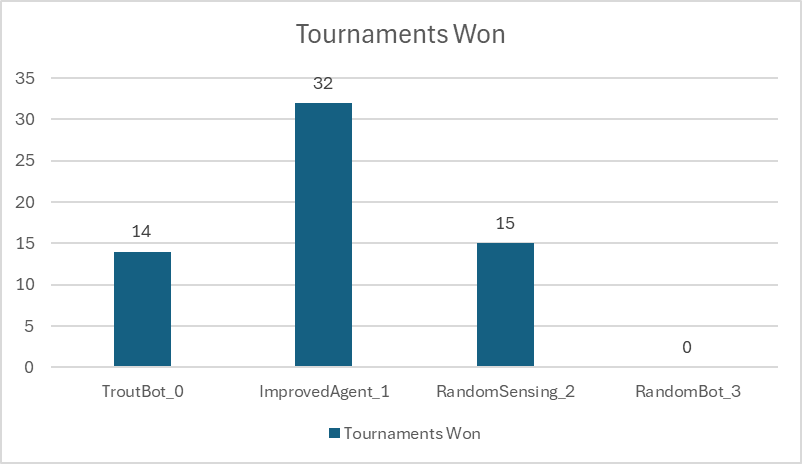
\includegraphics[width=0.6\textwidth]{tournamentTotal.png}
\caption{Tallied results of the round-robin tournament}
\label{fig:tournamentTotal}
\end{figure}

\begin{table}[H]
\centering
\caption{Results of Round-Robin Tournament}
\label{tab:results}
\begin{tabular}{|l|c|c|c|c|c|}
\hline
\textbf{Bot} & \textbf{Tournaments Won} & \textbf{Round Wins} & \textbf{Wins as White} & \textbf{Wins as Black} & \textbf{Round Draws} \\ \hline
TroutBot\_0 & 14 & 182 & 88 & 94 & 0 \\ \hline
ImprovedAgent\_1 & 32 & 227 & 108 & 119 & 2 \\ \hline
RandomSensing\_2 & 15 & 182 & 83 & 99 & 2 \\ \hline
RandomBot\_3 & 0 & 7 & 5 & 2 & 0 \\ \hline
\end{tabular}
\end{table}

\section{Improvements}

\subsection{RandomSensing}

RandomSensing's strategic performance was hindered by its reliance on random sensing, limiting its strategic adaptability and predictive capabilities. This approach led to suboptimal decision-making and reduced strategic effectiveness in Reconnaissance Blind Chess.

\subsection{Key Improvements Implemented for ImprovedAgent}

To enhance the agent's strategic capabilities, we implemented several key improvements to the sensing mechanism:

\subsubsection{Prioritized Sensing}

The ImprovedAgent incorporates a prioritized sensing algorithm to intelligently select the most advantageous square to sense during the Reconnaissance Blind Chess game. This algorithm aims to gather valuable information about the opponent's piece positions by prioritizing squares that have a higher potential for capturing enemy pieces in their surrounding region.

The prioritized sensing algorithm is implemented in the \texttt{choose\_sense} method of the ImprovedAgent class. The algorithm works as follows:

\begin{enumerate}
    \item If the opponent has captured one of the agent's pieces in the previous move, the algorithm focuses on a $3\times3$ region around the captured square. It adjusts the rank and file of the captured square to ensure that the $3\times3$ region falls within the bounds of the board, even if the captured square is on the edge or corner. The algorithm then returns the adjusted square as the chosen sense action.
    
    \item If no piece has been captured, the algorithm iterates through the set of possible board states (\texttt{self.possible\_fens}) and the available sense actions (\texttt{sense\_actions}).
    
    \item For each square in \texttt{sense\_actions} that falls within the inner region of the board (to avoid selecting squares on the edges or corners), the algorithm evaluates the potential benefit of sensing that square by calling the \texttt{evaluate\_region} function.
    
    \item The \texttt{evaluate\_region} function calculates the value of the square by summing up the piece values of the opponent's pieces in the surrounding $3\times3$ region. The piece values are defined in the \texttt{piece\_values} dictionary, with each piece type assigned a corresponding numerical value (e.g., pawn: 1, knight: 3, bishop: 3, rook: 5, queen: 9, king: 10).
    
    \item The algorithm keeps track of the maximum value found so far (\texttt{max\_value}) and the corresponding best square (\texttt{best\_square}).
    
    \item After evaluating all the squares, the algorithm returns the \texttt{best\_square} as the chosen sense action.
\end{enumerate}

\begin{figure}[H]
  \centering
  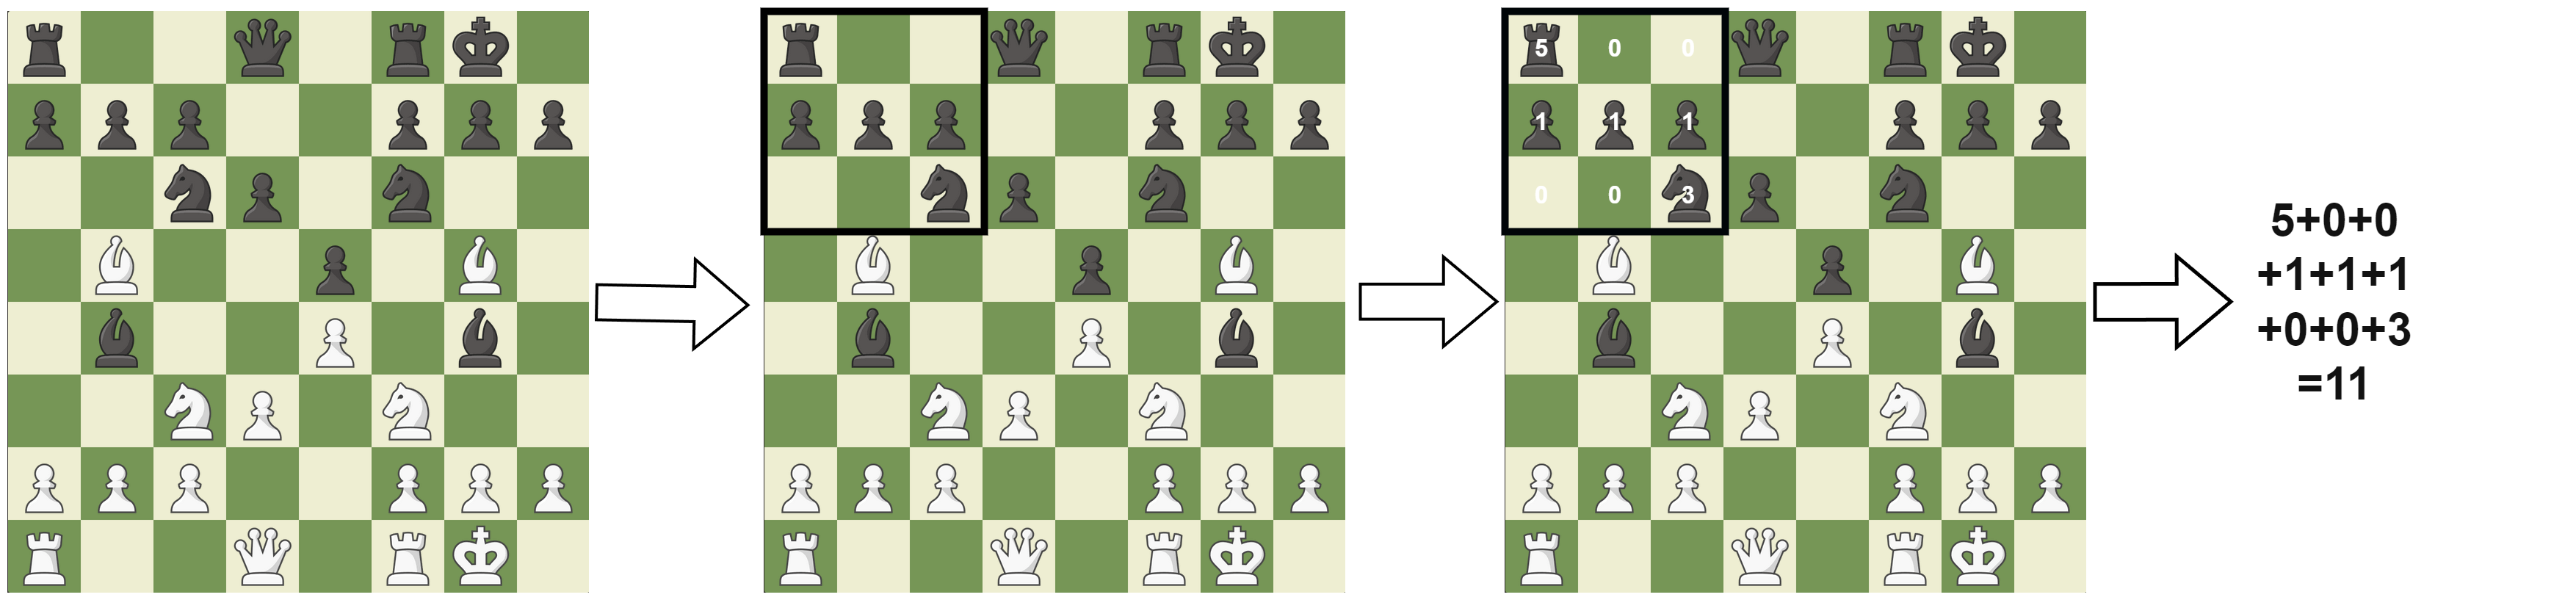
\includegraphics[width=0.6\textwidth]{pieces.png}
  \caption{Visualization of the piece values used in prioritized sensing}
  \label{fig:pieces}
\end{figure}

We experimented with different piece values, particularly the king's value, to optimize the sensing prioritization. For example, when the king's value was set to 2, the ImprovedAgent achieved a win rate of 0.659, while the TroutBot's win rate was 0.340. Adjusting the king's value to 0 resulted in a win rate of 0.571 for the ImprovedAgent and 0.428 for the TroutBot. Further increasing the king's value to 10 led to the ImprovedAgent's win rate improving to 0.664, while the TroutBot's win rate decreased to 0.335. These results, summarized in Table \ref{tab:win_rates}, demonstrate the impact of prioritized sensing and the importance of tuning piece values to optimize the agent's performance. Since the king value of 10 showed the most significant improvement, we conducted extensive testing on this configuration, running numerous games in parallel on the MSL cluster through our pipeline to obtain an accurate understanding of its performance.

\begin{table}[h]
  \centering
  \begin{tabular}{|c|c|c|c|}
  \hline
  \textbf{King Value} & \textbf{TroutBot Win Rate} & \textbf{ImprovedAgent Win Rate} & \textbf{Total Games Averaged on} \\
  \hline
  2 & 0.340 & 0.659 & 555 \\
  \hline
  0 & 0.428 & 0.571 & 810 \\
  \hline
  10 & 0.335 & 0.664 & 7868 \\
  \hline
  \end{tabular}
  \caption{Win rates for TroutBot and ImprovedAgent with different king values in prioritized sensing.}
  \label{tab:win_rates}
\end{table}

The rationale behind this approach is to prioritize sensing squares that are more likely to provide valuable information about the opponent's piece positions, specifically those squares where capturing enemy pieces is possible. By focusing on squares with higher potential for capturing, the agent can gather strategic insights and make more informed decisions during the game.

\subsubsection{Captured Piece Information}
When the opponent captures one of the agent's pieces, the agent utilizes this information to narrow down the possible board states. It identifies the captured square and focuses on a 3x3 region around that square, handling cases where the captured square is on the edges and corners of the board, mainting a full 3x3 sense region to get the most amount of information possible. The agent then filters out board states where the captured piece is still present in this 3x3 region, significantly reducing the search space.

\subsubsection{Sense Result Filtering}
After sensing a square, the agent filters out board states that do not match the sense result, further refining the possible board states. This allows the agent to maintain a more accurate representation of the board state based on the information gathered through sensing.

\subsubsection{Check Handling}
When the enemy king is in check, the ImprovedAgent prioritizes moves that capture the enemy king or moves that get the king out of check. For each possible board state, the agent identifies if the enemy king is under attack and, if so, attempts to find a move that captures the enemy king or a legal move that does not leave the king in check. This strategic consideration improves the agent's ability to handle check scenarios effectively.

\section{Conclusion}
By incorporating these techniques, the number of possible board states that the agent needs to consider is drastically reduced compared to a random sensing approach. This reduction in the search space allows the Stockfish engine, which is used for move evaluation, to spend more time analyzing each remaining board state and explore deeper variations. As a result, Stockfish can provide more accurate and informed move evaluations, enabling the ImprovedAgent to make better strategic decisions and improve its overall performance in Reconnaissance Blind Chess.


    
  
\end{document}